\documentclass{article}
\usepackage[paperheight = 85cm, paperwidth = 107cm, margin=1cm, heightrounded]{geometry}
\usepackage{physics}
\usepackage{tikz}
\usepackage{amsmath}
\usetikzlibrary{mindmap}

\begin{document}
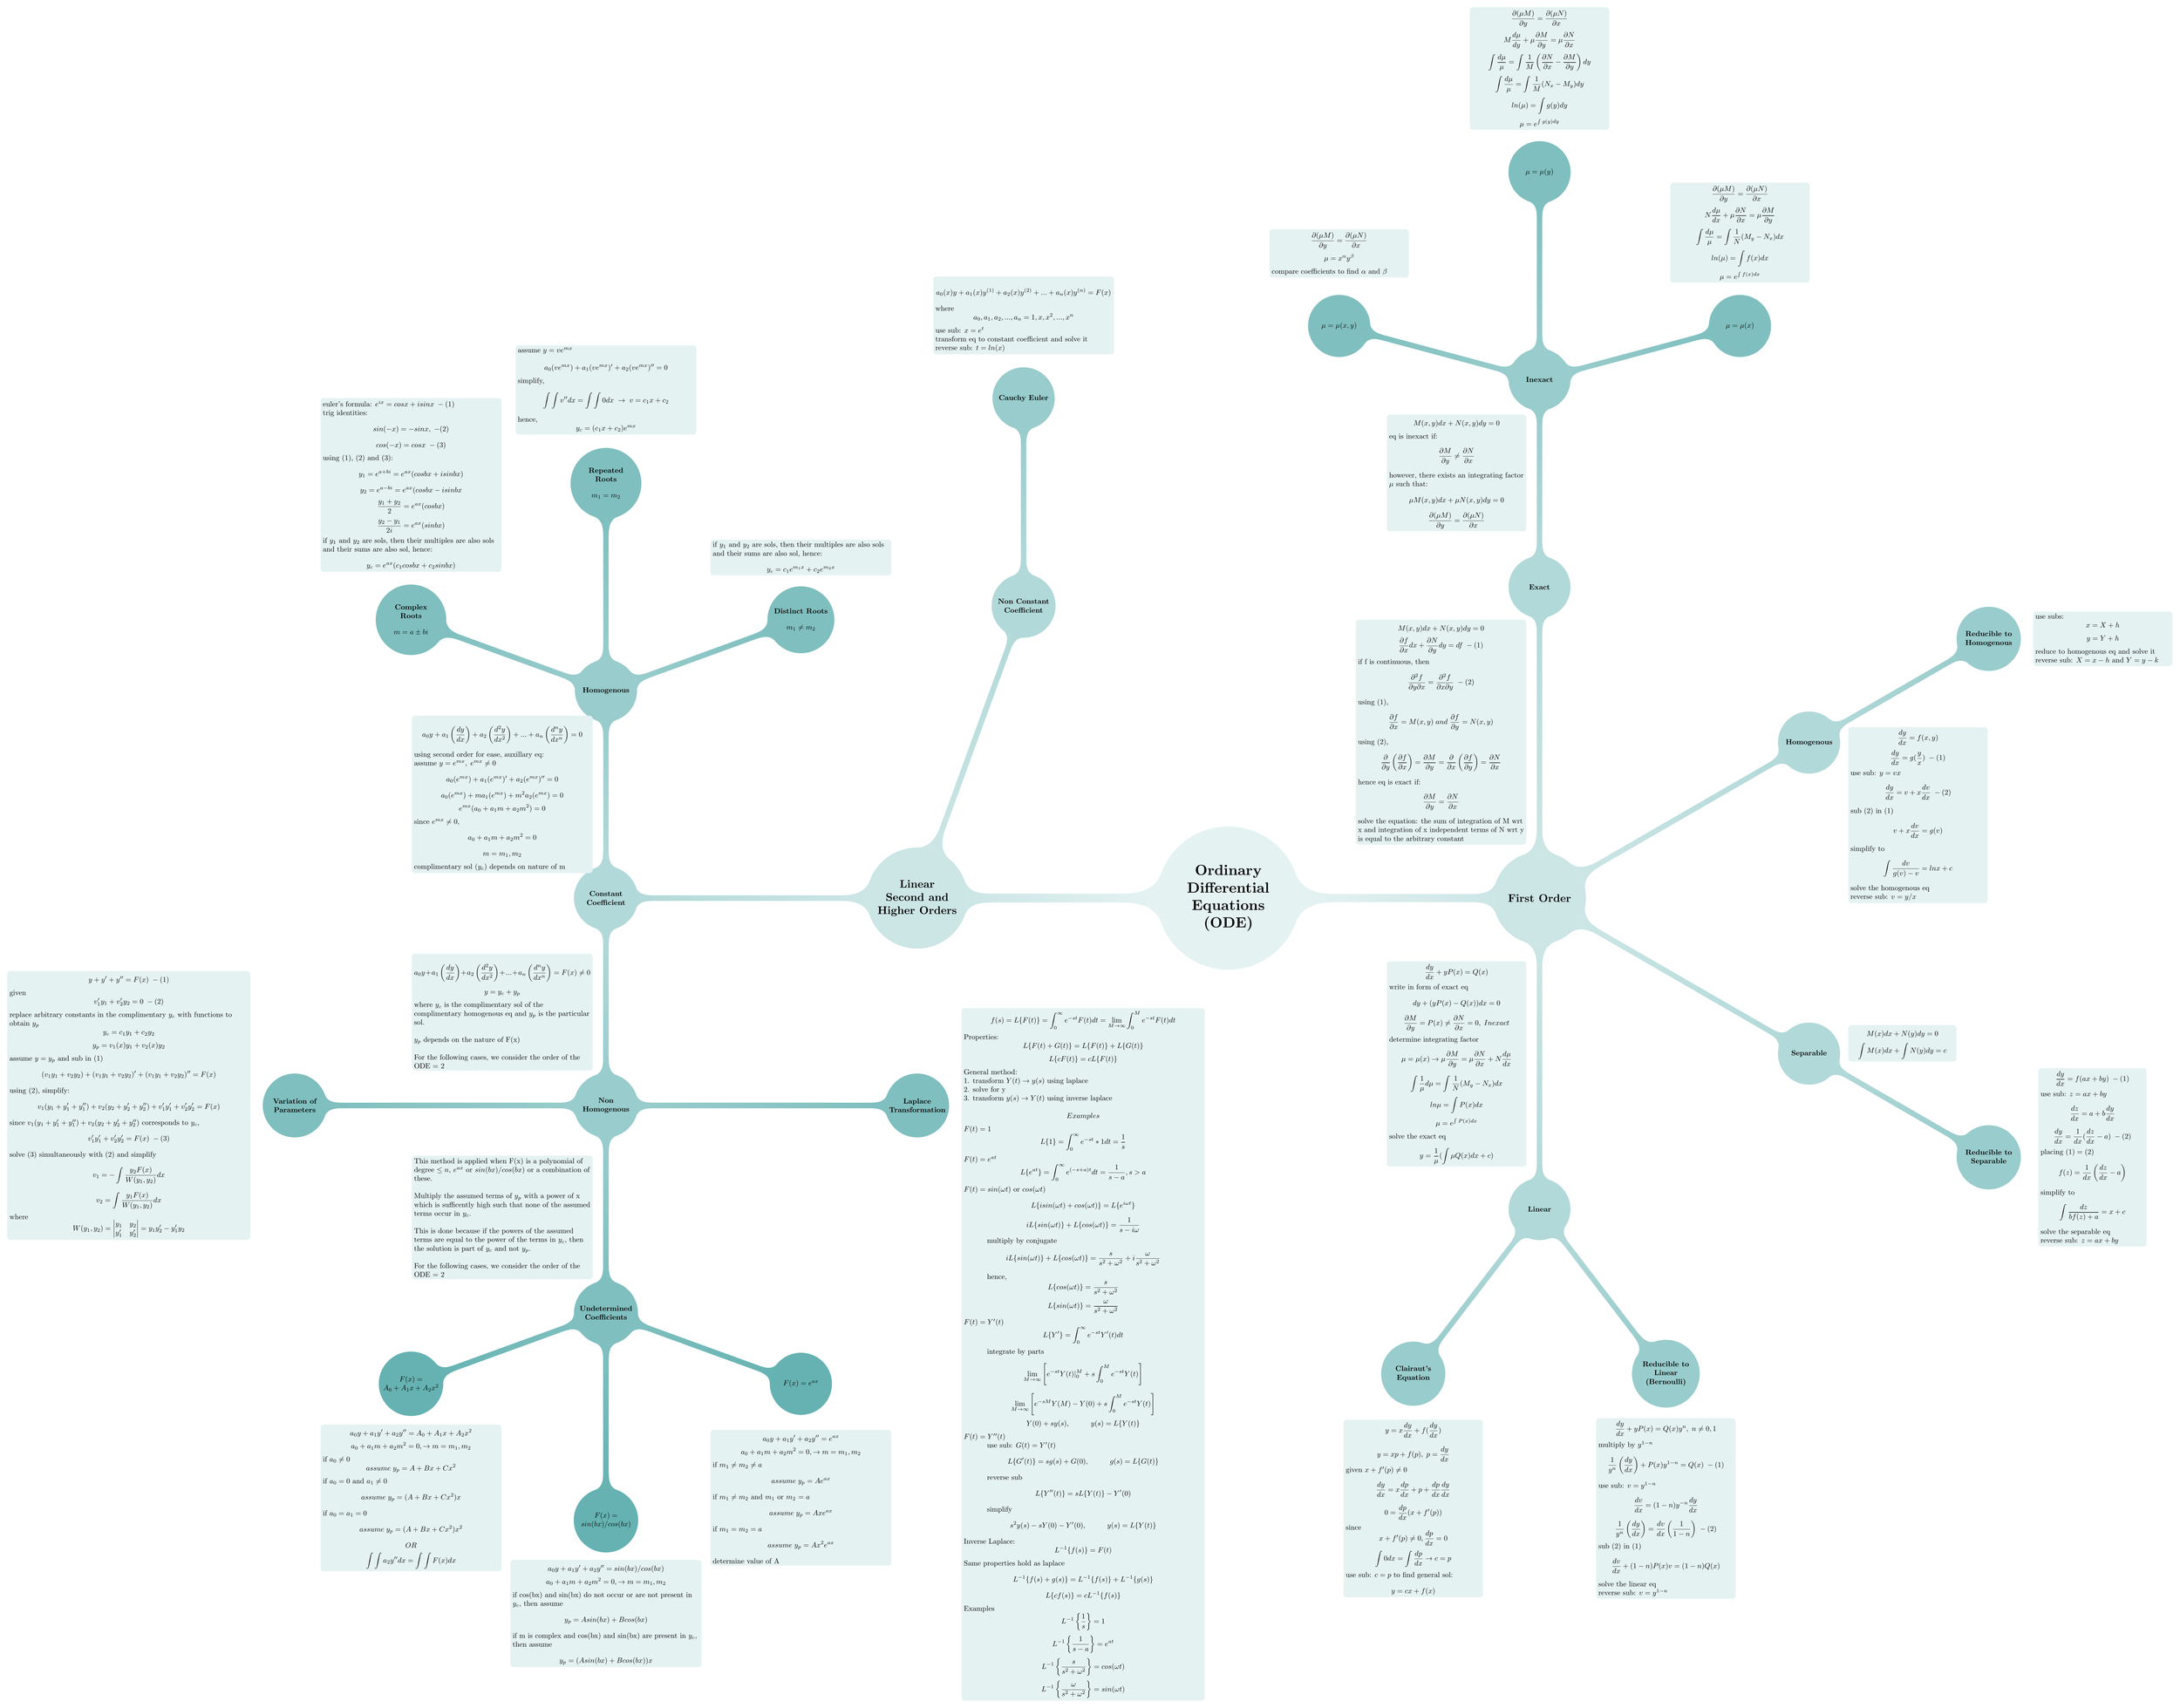
\begin{tikzpicture}
	[grow cyclic, text width = 2.7cm, align = flush center, 
	every node/.style = concept, concept color = teal!10, rotate = 90,
	level 1/.style = {level distance = 15cm, concept color = teal!20},
	level 2/.style = {level distance = 15cm, concept color = teal!30},
	level 3/.style = {level distance = 10cm, concept color = teal!40},
	level 4/.style = {level distance = 10cm, concept color = teal!50},
	level 5/.style = {level distance = 10cm, concept color = teal!60}]

\node [scale = 2] {\textbf{Ordinary Differential Equations \\ (ODE)}}
	child [sibling angle = 180] {node [scale = 1.5] {\textbf{First Order}}
		child [sibling angle = 60] {node (lin) {\textbf{Linear}}
			child [sibling angle = 75] {node (non-lin) {\textbf{Clairaut's Equation}}}
			child [sibling angle = 75] {node (red-lin) {\textbf{Reducible to Linear \\ (Bernoulli)}}}
		}
		child [sibling angle = 60] {node (sep) {\textbf{Separable}}
			child {node (red-sep) {\textbf{Reducible to Separable}}}
		}
		child [sibling angle = 60] {node (1-homo) {\textbf{Homogenous}}
			child {node (1-red-homo) {\textbf{Reducible to Homogenous}}}
		}
		child [sibling angle = 60] {node (exact) {\textbf{Exact}}
			child {node (inexact) {\textbf{Inexact}}
				child [sibling angle = 75] {node (x) {$\mu = \mu (x)$}}
				child [sibling angle = 75] {node (y) {$\mu = \mu (y)$}}
				child [sibling angle = 75] {node (xy) {$\mu = \mu (x,y)$}}
			}
		}
	}
	child [sibling angle = 180] {node [scale = 1.5] {\textbf{Linear \\ Second and Higher Orders}}
		child [clockwise from = -110, level distance = 15cm] {node {\textbf{Non Constant Coefficient}}
			child [clockwise from = -90] {node (CE) {\textbf{Cauchy Euler}}}
		}
		child [sibling angle = 0] {node {\textbf{Constant Coefficient}}
			child [sibling angle = 180] {node (2-homo) {\textbf{Homogenous}}
				child [sibling angle = 70] {node (distinct) {\textbf{Distinct Roots} $$m_1 \neq m_2$$}}
				child [sibling angle = 70] {node (repeat) {\textbf{Repeated Roots} $$m_1 = m_2$$}}
				child [sibling angle = 70]{node (complex) {\textbf{Complex Roots} $$m = a \pm b i$$}}
			}
			child [sibling angle = 180] {node (2-non-homo) {\textbf{Non Homogenous}}
				child [sibling angle = 90, level distance = 15cm] {node (VP) {\textbf{Variation of Parameters}}}
				child [sibling angle = 90] {node (UC) {\textbf{Undetermined Coefficients}}
					child [sibling angle = 70] {node (pol) {$F(x) = A_0 + A_1x + A_2x^2$}}
					child [sibling angle = 70] {node (trig) {$F(x) = sin(bx)/cos(bx)$}}
					child [sibling angle = 70] {node (exp) {$F(x) = e^{ax}$}}
				}
				child [sibling angle = 90, level distance = 15cm] {node (LT) {\textbf{Laplace \\ Transformation}}}
			}
		}
	}
;

\node[annotation, centered, font=, xshift = 4.5cm, yshift = 0.5cm, text width = 5cm] at (sep)
	{$$M(x)dx + N(y)dy = 0$$
	$$\int M(x)dx + \int N(y)dy = c$$
	};

\node[annotation, centered, font=, xshift = 5cm, text width = 5cm] at (red-sep)
	{$$\frac{dy}{dx} = f(ax+by) \hspace{0.1cm} -(1)$$ 
	use sub: $z = ax + by$
	$$\frac{dz}{dx} = a + b\frac{dy}{dx}$$
	$$\frac{dy}{dx} = \frac{1}{dx} (\frac{dz}{dx} - a) \hspace{0.1cm} -(2)$$
	placing $(1) = (2)$
	$$f(z) = \frac{1}{dx} \left(\frac{dz}{dx} - a\right)$$
	simplify to
	$$\int \frac{dz}{bf(z) + a} = x + c$$
	solve the separable eq \\
	reverse sub: $z = ax + by$
	};
	
\node[annotation, centered, font=, xshift = -4cm, yshift = 7cm, text width = 6.5cm] at (lin)
	{$$\frac{dy}{dx} + yP(x) = Q(x)$$
	write in form of exact eq
	$$dy + (yP(x) - Q(x))dx = 0$$
	$$\frac{\partial M}{\partial y} = P(x) \neq \frac{\partial N}{\partial x} = 0, \hspace{0.1cm} Inexact$$
	determine integrating factor
	$$\mu = \mu (x) \rightarrow \mu \frac{\partial M}{\partial y} = \mu \frac{\partial N}{\partial x} + N \frac{d\mu}{dx}$$
	$$\int \frac{1}{\mu} d\mu = \int \frac{1}{N} (M_y - N_x) dx$$
	$$ln\mu = \int P(x) dx$$
	$$\mu = e^{\int P(x) dx}$$
	solve the exact eq
	$$y = \frac{1}{\mu} (\int \mu Q(x) dx + c)$$
	};

\node[annotation, centered, font=, yshift = -6.5cm, text width = 6.5cm] at (red-lin)
	{$$\frac{dy}{dx} + yP(x) = Q(x)y^n, \hspace{0.1cm} n \neq 0,1$$
	multiply by $y^{1-n}$
	$$\frac{1}{y^n}\left (\frac{dy}{dx}\right) + P(x)y^{1-n} = Q(x) \hspace{0.1cm} -(1)$$
	use sub: $v = y^{1-n}$
	$$\frac{dv}{dx} = (1-n)y^{-n} \frac{dy}{dx}$$
	$$\frac{1}{y^n}\left(\frac{dy}{dx}\right) = \frac{dv}{dx} \left(\frac{1}{1-n}\right) \hspace{0.1cm} -(2)$$
	sub (2) in (1)
	$$\frac{dv}{dx} + (1-n)P(x)v = (1-n)Q(x)$$
	solve the linear eq \\
	reverse sub: $v = y^{1-n}$
	};

\node[annotation, centered, font=, yshift = -6.5cm, text width = 6.5cm] at (non-lin)
	{\textbf{$$y = x\frac{dy}{dx} + f(\frac{dy}{dx})$$}
	$$y = xp + f(p), \hspace{0.1cm} p = \frac{dy}{dx}$$
	given $x + f'(p) \neq 0$
	$$\frac{dy}{dx} = x\frac{dp}{dx} + p + \frac{dp}{dx} \frac{dy}{dx}$$
	$$0 = \frac{dp}{dx} (x + f'(p))$$
	since $$x + f'(p) \neq 0, \frac{dp}{dx} = 0$$
	$$\int 0 dx = \int \frac{dp}{dx} \rightarrow c = p$$
	use sub: $c = p$ to find general sol:
	$$y = cx + f(x)$$
	};

\node[annotation, centered, font=, yshift = -7cm, xshift = -4.75cm, text width = 8cm] at (exact)
	{$$M(x,y)dx + N(x,y)dy = 0$$
	$$\frac{\partial f}{\partial x} dx + \frac{\partial N}{\partial y} dy = df \hspace{0.1cm} -(1)$$
	if f is continuous, then
	$$\frac{\partial^2 f}{\partial y \partial x} = \frac{\partial^2 f}{\partial x \partial y} \hspace{0.1cm} -(2)$$
	using (1),
	$$\frac{\partial f}{\partial x} = M(x,y) \hspace{0.1cm} and \hspace{0.1cm} \frac{\partial f}{\partial y} = N(x,y)$$
	using (2),
	$$\frac{\partial}{\partial y}\left(\frac{\partial f}{\partial x}\right) = \frac{\partial M}{\partial y} = \frac{\partial}{\partial x}\left(\frac{\partial f}{\partial y}\right) = \frac{\partial N}{\partial x}$$
	hence eq is exact if:
	$$\frac{\partial M}{\partial y} = \frac{\partial N}{\partial x}$$
	solve the equation: the sum of integration of M wrt x and integration of x independent terms of N wrt y is equal to the arbitrary constant
	};

\node[annotation, centered, font=, yshift = -4.5cm, xshift = -4cm, text width = 6.5cm] at (inexact)
	{$$M(x,y)dx + N(x,y)dy = 0$$
	eq is inexact if:
	$$\frac{\partial M}{\partial y} \neq \frac{\partial N}{\partial x}$$
	however, there exists an integrating factor $\mu$ such that:
	$$\mu M(x,y)dx + \mu N(x,y)dy = 0$$
	$$\frac{\partial (\mu M)}{\partial y} = \frac{\partial (\mu N)}{\partial x}$$
	};

\node[annotation, centered, font=, yshift = 4.5cm, text width = 6.5cm] at (x)
	{$$\frac{\partial (\mu M)}{\partial y} = \frac{\partial (\mu N)}{\partial x}$$
	$$N \frac{d\mu}{dx} + \mu \frac{\partial N}{\partial x} = \mu \frac{\partial M}{\partial y}$$
	$$\int \frac{d \mu}{\mu} = \int \frac{1}{N}(M_y - N_x)dx$$
	$$ln(\mu) = \int f(x)dx$$
	$$\mu = e^{\int f(x)dx}$$};

\node[annotation, centered, font=, yshift = 5cm, text width = 6.5cm] at (y)
	{$$\frac{\partial (\mu M)}{\partial y} = \frac{\partial (\mu N)}{\partial x}$$
	$$M \frac{d\mu}{dy} + \mu \frac{\partial M}{\partial y} = \mu \frac{\partial N}{\partial x}$$
	$$\int \frac{d \mu}{\mu} = \int \frac{1}{M}\left(\frac{\partial N}{\partial x} - \frac{\partial M}{\partial y}\right)dy$$
	$$\int \frac{d \mu}{\mu} = \int \frac{1}{M}(N_x - M_y)dy$$
	$$ln(\mu) = \int g(y)dy$$
	$$\mu = e^{\int g(y)dy}$$
	};

\node[annotation, centered, font=, yshift = 3.5cm, text width = 6.5cm] at (xy)
	{$$\frac{\partial (\mu M)}{\partial y} = \frac{\partial (\mu N)}{\partial x}$$
	$$\mu = x^{\alpha} y^{\beta}$$
	compare coefficients to find $\alpha$ and $\beta$
	};

\node[annotation, centered, font=, xshift = 5.25cm, yshift = -3.5cm, text width = 6.5cm] at (1-homo)
	{$$\frac{dy}{dx} = f(x,y)$$ 
	$$\frac{dy}{dx} = g(\frac{y}{x}) \hspace{0.1cm} -(1)$$ 
	use sub: $y = vx$
	$$\frac{dy}{dx} = v + x\frac{dv}{dx} \hspace{0.1cm} -(2)$$
	sub (2) in (1)
	$$v + x\frac{dv}{dx} = g(v)$$
	simplify to
	$$\int \frac{dv}{g(v)-v} = lnx + c$$
	solve the homogenous eq\\
	reverse sub: $v = y/x$
	};

\node[annotation, centered, font=, xshift = 5.5cm, text width = 6.5cm] at (1-red-homo)
	{use subs:
	$$x = X + h$$
	$$y = Y + h$$
	reduce to homogenous eq and solve it
	reverse sub: $X = x - h$ and $Y = y - k$
	};

\node[annotation, centered, font=, yshift = 4cm, text width = 8.5cm] at (CE)
	{$$a_0(x)y + a_1(x)y^{(1)} + a_2(x)y^{(2)} + ... + a_n(x)y^{(n)}= F(x)$$
	where 
	$$a_0, a_1, a_2, ..., a_n = 1,x,x^2, ..., x^n$$
	use sub: $x = e^t$ \\
	transform eq to constant coefficient and solve it \\
	reverse sub: $t = ln(x)$
	};

\node[annotation, centered, font=, yshift = -5cm, xshift = -5cm, text width = 8.5cm] at (2-homo)
	{$$a_0y + a_1\left(\frac{dy}{dx}\right) + a_2\left(\frac{d^2y}{dx^2}\right) + ... + a_n\left(\frac{d^ny}{dx^n}\right)= 0$$
	using second order for ease, auxillary eq: \\
	assume $y = e^{mx}, \hspace{0.1cm} e^{mx} \neq 0$
	$$a_0(e^{mx}) + a_1(e^{mx})' + a_2(e^{mx})'' = 0$$
	$$a_0(e^{mx}) + ma_1(e^{mx}) + m^2a_2(e^{mx}) = 0$$
	$$e^{mx}(a_0 + a_1m + a_2m^2) = 0$$
	since $e^{mx} \neq 0$,
	$$a_0 + a_1m + a_2m^2 = 0$$
	$$m = m_1, m_2$$
	complimentary sol ($y_c$) depends on nature of m
	};

\node[annotation, centered, font=, yshift = 3cm, text width = 8.5cm] at (distinct)
	{if $y_1$ and $y_2$ are sols, then their multiples are also sols and their sums are also sol, hence:
	$$y_c = c_1e^{m_1x} + c_2e^{m_2x}$$
	};

\node[annotation, centered, font=, yshift = 4.5cm, text width = 8.5cm] at (repeat)
	{assume $y = ve^{mx}$ \\
	$$a_0(ve^{mx}) + a_1(ve^{mx})' + a_2(ve^{mx})'' = 0$$
	simplify,
	$$\int \int v'' dx = \int \int 0 dx \hspace{0.1cm} \rightarrow \hspace{0.1cm} v = c_1x + c_2$$
	hence,
	$$y_c = (c_1x + c_2)e^{mx}$$
	};

\node[annotation, centered, font=, yshift = 6.5cm, text width = 8.5cm] at (complex)
	{euler's formula: $e^{ix} = cosx + i sinx \hspace{0.1cm} -(1)$ \\
	trig identities:
	$$sin(-x) = -sinx, \hspace{0.1cm} -(2)$$
	$$cos(-x) = cosx \hspace{0.1cm} -(3)$$
	using (1), (2) and (3):
	$$y_1 = e^{a+bi} = e^{ax} (cosbx + i sinbx)$$
	$$y_2 = e^{a - bi} = e^{ax} (cosbx - i sinbx$$
	$$\frac{y_1+y_2}{2} = e^{ax}(cosbx)$$
	$$\frac{y_2-y_1}{2i} = e^{ax}(sinbx)$$
	if $y_1$ and $y_2$ are sols, then their multiples are also sols and their sums are also sol, hence:
	$$y_c = e^{ax}(c_1cosbx + c_2sinbx)$$
	};	

\node[annotation, centered, font=, xshift = -5cm, yshift = 4.5cm, text width = 8.5cm] at (2-non-homo)
	{$$a_0y + a_1\left(\frac{dy}{dx}\right) + a_2\left(\frac{d^2y}{dx^2}\right) + ... + a_n\left(\frac{d^ny}{dx^n}\right) = F(x) \neq 0$$
	$$y = y_c + y_p$$ 
	where $y_c$ is the complimentary sol of the complimentary homogenous eq and $y_p$ is the particular sol. \\ \hspace{10cm}
	$y_p$ depends on the nature of F(x) \\ \hspace{10cm}
	For the following cases, we consider the order of the ODE = 2
	};

\node[annotation, centered, font=, xshift = -5cm, yshift = 4.6cm, text width = 8.5cm] at (UC)
	{This method is applied when F(x) is a polynomial of degree $\leq n$, $e^{ax}$ or $sin(bx)/cos(bx)$ or a combination of these. \\ \hspace{10cm}
	Multiply the assumed terms of $y_p$ with a power of x which is sufficently high such that none of the assumed terms occur in $y_c$. \\ \hspace{10cm}
	This is done because if the powers of the assumed terms are equal to the power of the terms in $y_c$, then the solution is part of $y_c$ and not $y_p$. \\ \hspace{10cm}
	For the following cases, we consider the order of the ODE = 2
	};

\node[annotation, centered, font=, yshift = -5.5cm, text width = 8.5cm] at (exp)
	{$$a_0y + a_1y' + a_2y'' = e^{ax}$$
	$$a_0 + a_1m + a_2m^2 = 0, \rightarrow m = m_1, m_2$$
	\\ if $m_1 \neq m_2 \neq a$
	$$assume \hspace{0.1cm} y_p = Ae^{ax}$$
	if $m_1 \neq m_2$ and $m_1$ or $m_2$ $=a$ 
	$$assume \hspace{0.1cm} y_p = Axe^{ax}$$
	if $m_1 = m_2 = a$
	$$assume \hspace{0.1cm} y_p = Ax^2e^{ax}$$
	determine value of A
	};

\node[annotation, centered, font=, yshift = -4.5cm, text width = 9cm] at (trig)
	{$$a_0y + a_1y' + a_2y'' = sin(bx) / cos(bx)$$
	$$a_0 + a_1m + a_2m^2 = 0, \rightarrow m = m_1, m_2$$
	if cos(bx) and sin(bx) do not occur or are not present in $y_c$, then assume
	$$y_p = Asin(bx) + Bcos(bx)$$
	if m is complex and cos(bx) and sin(bx) are present in $y_c$, then assume
	$$ y_p = (Asin(bx) + Bcos(bx))x$$
	};

\node[annotation, centered, font=, yshift = -5.5cm, text width = 8.5cm] at (pol)
	{$$a_0y + a_1y' + a_2y'' = A_0 + A_1x + A_2x^2$$
	$$a_0 + a_1m + a_2m^2 = 0, \rightarrow m = m_1, m_2$$
	if $a_0 \neq 0$ 
	$$assume \hspace{0.1cm} y_p = A + Bx + Cx^2$$
	if $a_0 = 0$ and $a_1 \neq 0$
	$$assume \hspace{0.1cm} y_p = (A + Bx + Cx^2)x$$
	if $a_0 = a_1 = 0$
	$$assume \hspace{0.1cm} y_p = (A + Bx + Cx^2)x^2$$
	$$OR$$
	$$\int \int a_2y'' dx= \int \int F(x) dx$$
	};

\node[annotation, centered, font=, xshift = -8cm, text width = 11.5cm] at (VP)
	{$$y + y' + y'' = F(x) \hspace{0.1cm} -(1)$$
	given 
	$$v_1'y_1 + v_2'y_2 = 0 \hspace{0.1cm} -(2)$$
	replace arbitrary constants in the complimentary $y_c$ with functions to obtain $y_p$ 
	$$y_c = c_1y_1 + c_2y_2$$
	$$y_p = v_1(x)y_1 + v_2(x)y_2$$
	assume $y = y_p$ and sub in (1)
	$$(v_1y_1 + v_2y_2) + (v_1y_1 + v_2y_2)' + (v_1y_1 + v_2y_2)'' = F(x)$$
	using (2), simplify:
	$$v_1(y_1 + y_1' + y_1'') + v_2(y_2 + y_2' + y_2'') + v_1'y_1' + v_2'y_2' = F(x)$$
	since $v_1(y_1 + y_1' + y_1'') + v_2(y_2 + y_2' + y_2'')$ corresponds to $y_c$, 
	$$v_1'y_1' + v_2'y_2' = F(x) \hspace{0.1cm} -(3)$$
	solve (3) simultaneously with (2) and simplify
	$$v_1 = - \int \frac{y_2F(x)}{W(y_1,y_2)} dx$$
	$$v_2 = \int \frac{y_1F(x)}{W(y_1,y_2)} dx$$
	where
	$$W(y_1,y_2) =  \mdet{ y_1 & y_2 \\ y_1' & y_2' } = y_1y_2' - y_1'y_2$$
	};

\node[annotation, centered, font=, xshift = 8cm, yshift = -12cm, text width = 11.5cm] at (LT)
	{$$f(s) = L\{F(t)\} = \int_{0}^{\infty} e^{-st}F(t) dt = \lim\limits_{M \rightarrow \infty} \int_{0}^{M} e^{-st} F(t)dt$$
	Properties:
	$$L\{F(t) + G(t)\} = L\{F(t)\} + L\{G(t)\}$$
	$$L\{cF(t)\} = cL\{F(t)\}$$
	General method: \\
	1. transform $Y(t) \rightarrow y(s)$ using laplace \\
	2. solve for y \\
	3. transform $y(s) \rightarrow Y(t)$ using inverse laplace\\
	$$Examples$$
	$F(t) = 1$
	$$L\{1\} = \int_{0}^{\infty} e^{-st} * 1 dt = \frac{1}{s}$$
	$F(t) = e^{at}$
	$$L\{e^{at}\} = \int_{0}^{\infty} e^{(-s+a)t} dt = \frac{1}{s-a}, s > a$$
	$F(t) = sin(\omega t)$ or $cos(\omega t)$
	$$L\{i sin(\omega t) + cos(\omega t)\} = L\{e^{i \omega t}\}$$
	$$i L\{sin(\omega t)\} + L\{cos(\omega t)\} = \frac{1}{s-i \omega}$$
	$\hspace{1cm}$ multiply by conjugate
	$$i L\{sin(\omega t)\} + L\{cos(\omega t)\} = \frac{s}{s^2 + \omega^2} + i \frac{\omega}{s^2 + \omega^2}$$
	$\hspace{1cm}$ hence,
	$$L\{cos(\omega t)\} = \frac{s}{s^2 + \omega^2}$$
	$$L\{sin(\omega t)\} = \frac{\omega}{s^2 + \omega^2}$$
	$F(t) = Y'(t)$
	$$L\{Y'\} = \int_{0}^{\infty} e^{-st} Y'(t)dt$$
	$\hspace{1cm}$ integrate by parts
	$$\lim\limits_{M \rightarrow \infty}  \left[e^{-st} Y(t) |^M_0 + s\int_{0}^{M} e^{-st} Y(t)\right]$$
	$$\lim\limits_{M \rightarrow \infty} \left[e^{-sM} Y(M) -  Y(0) + s\int_{0}^M e^{-st} Y(t)\right]$$
	$$Y(0) + sy(s), \hspace{1cm} y(s) = L\{Y(t)\}$$
	$F(t) = Y''(t)$ \\
	$\hspace{1cm}$ use sub: $G(t) = Y'(t)$
	$$L\{G'(t)\} = sg(s) + G(0), \hspace{1cm} g(s) = L\{G(t)\}$$
	$\hspace{1cm}$ reverse sub
	$$L\{Y''(t)\} = sL\{Y(t)\} - Y'(0)$$
	$\hspace{1cm}$ simplify
	$$s^2y(s) - sY(0) - Y'(0), \hspace{1cm} y(s) = L\{Y(t)\}$$
	Inverse Laplace:
	$$L^{-1}\{f(s)\} = F(t)$$
	Same properties hold as laplace
	$$L^{-1}\{f(s) + g(s)\} = L^{-1}\{f(s)\} + L^{-1}\{g(s)\}$$
	$$L\{cf(s)\} = cL^{-1}\{f(s)\}$$
	Examples
	$$L^{-1}\left\{\frac{1}{s}\right\} = 1$$
	$$L^{-1}\left\{\frac{1}{s-a}\right\} = e^{at}$$
	$$L^{-1}\left\{\frac{s}{s^2 + \omega^2}\right\} = cos(\omega t)$$
	$$L^{-1}\left\{\frac{\omega}{s^2 + \omega^2}\right\} = sin(\omega t)$$
	};

\end{tikzpicture}
\end{document}	
